\documentclass[a4paper]{scrartcl}

\usepackage[ngerman]{babel}
\usepackage[final]{microtype}
\usepackage[T1]{fontenc}
\linespread{1.05}

\usepackage[inner=3cm,outer=2cm,top=3cm,bottom=3cm,foot=1.75cm]{geometry}
\setlength{\columnsep}{20pt}

\usepackage{xcolor}
\usepackage{lmodern}
\usepackage{amsmath, amsthm, amssymb, mathtools}
\usepackage{unicode-math}
\usepackage{fontspec}
\defaultfontfeatures{Ligatures=TeX,Scale=MatchLowercase}

\let\emptyset\varnothing

\usepackage{url}
\usepackage{graphicx}

\usepackage{enumitem}
\setlist{nolistsep}
\setlist[itemize]{noitemsep}

\setlength{\parindent}{0pt}
\setlength{\parskip}{6pt plus 2pt minus 1pt}

\usepackage[font=small]{caption}

\usepackage{abstract}
\renewcommand{\abstractnamefont}{\normalfont\bfseries}
\renewcommand{\abstracttextfont}{\normalfont\small}

\usepackage{titlesec}
\renewcommand\thesection{\Roman{section}}
\renewcommand\thesubsection{\roman{subsection}}
\titleformat{\section}[block]{\large\scshape\centering}{\thesection.}{1em}{}
\titleformat{\subsection}[block]{\large}{\thesubsection.}{1em}{}

\usepackage{hyperref}
\hypersetup{pdfborder={0 0 0},breaklinks=true}

\setlength{\emergencystretch}{3em}
\interfootnotelinepenalty=10000

\usepackage{titling}
\setlength{\droptitle}{-2\baselineskip}
\pretitle{\begin{center}\huge\bfseries}
\posttitle{\end{center}}
\renewcommand{\subtitle}[1]{%
  \posttitle{%
    \par\end{center}
    \begin{center}\Large\bfseries#1\end{center}
    \vskip0.5em}%
}

\usepackage[automark]{scrpage2}
\pagestyle{scrheadings}
\clearscrheadfoot
\rohead[]{\textsc{\leftmark}}
\lehead[]{\textsc{\leftmark}}
\rofoot[\pagemark]{\pagemark}
\lefoot[\pagemark]{\pagemark}

\makeatletter
  \newcommand\footnoteref[1]{\protected@xdef\@thefnmark{\ref{#1}}\@footnotemark}
\makeatother

\renewcommand{\arraystretch}{1.2}

\newcommand\e[1]{\begin{em}#1\end{em}}

\newcommand\q[1]{\glqq #1\grqq}

\newcommand\sq[1]{\glq #1\grq}

\newcommand\qq[1]{\glqq\e{#1}\grqq}

\newcommand\fnm[1]{\footnotemark[#1]\addtocounter{footnote}{1}}

\newcommand\g[4]{%
  \begin{figure}[!ht]
  \centering
  \includegraphics[width=#4\textwidth]{#1}
  \caption{#3\label{fig:#2}}
  \end{figure}}

\newcommand\todo[1]{\colorbox{yellow}{#1}}


\title{Spielbäume}
\def\titlehead{Spielbäume}
\subtitle{Proseminar Theoretische Informatik}
\author{Joschka Heinrich\thanks{joschka.heinrich@tu-dresden.de, PGP: \textsc{B40E 67C7 FF62 C860 7854 A778 6FB9 666F 1147 A401}}, TU Dresden}

\begin{document}
\maketitle



\section{Einführung}
Was sind Spielbäume und wozu können sie verwendet werden? In dieser Ausarbeitung wird das Konzept des Spielbaumes formal eingeführt und anhand des Spiels \e{Tic-Tac-Toe} beispielhaft erläutert. Mit der Erklärung des Alpha-Beta-Prunings als Optimierung des Minimax-Verfahrens wird eine Anwendung von Spielbäumen illustriert.


\section{Spielbäume}
Um im Folgenden mit Spielbäumen arbeiten zu können, führen wir das Konzept zunächst formal ein und definieren dazu unter anderem den Begriff des \e{Spiels}, der \e{Konfiguration} und des \e{Spielbaums}.


\subsection{Definition}

Alle folgenden Betrachtungen nehmen wir aus der Perspektive eines gewinnorientierten Spielers namens \textsc{Max} vor, der sich einer Anzahl Gegner gegenüber sieht. Es ist also das Ziel, Züge für \textsc{Max} so zu finden, dass dessen Gewinn maximiert, bzw. der Gewinn der Gegner minimiert wird. Wir gehen dabei davon aus, dass auch alle Gegner optimale Entscheidungen treffen. Wir vereinfachen die Betrachtung von Spielen, indem wir uns auf solche ohne Zufallskomponente, d.h. reine Strategiespiele mit vollkommener Information und Spiele mit zwei Kontrahenten -- \textsc{Max} und ein zweiter Spieler \textsc{Min} -- beschränken. Mit \q{der Gegner} ist also im Folgenden stets \textsc{Min} gemeint. 

Ein \textbf{Spiel} $S = (R,k_0,F)$ ist nun durch Regeln, in Form einer endlichen Menge $R$ von legalen Spielzügen (als Funktionen auf den Konfigurationen), eine Anfangskonfiguration $k_0 \in K$ und eine Reihe möglicher Endkonfigurationen $F \subset K$ gegeben, mit $K$, der Menge aller \e{zulässigen} Konfigurationen. Eine \textbf{Konfiguration} $k \in K$ repräsentiert dabei einen möglichen Zustand des Spieles, bestehend aus einer Beschreibung wiederum der Zustände aller relevanten Spielelemente (bspw. die Position der Zeichen auf dem Tic-Tac-Toe-Feld) inklusive des Spielers, der als nächster an der Reihe ist (bei uns entweder \textsc{Max} oder \textsc{Min}).

In Abgrenzung zur Menge der \e{legalen} Spielzüge können wir uns beliebige andere Spielzüge vorstellen, die zwar möglich, allerdings in dem betrachteten Spiel nicht erlaubt sind. Analog dazu sind über $K$ hinaus weitere Konfigurationen denkbar, die allerdings nicht zulässig sind, d.h. in einem regelkonformen Spiel niemals auftreten können. Dieser Zusammenhang wird in Abb.~\ref{fig:venn} veranschaulicht. 

Durch Anwenden eines legalen Spielzuges auf eine Konfiguration gelangen wir zu einer neuen Konfiguration. Ein legaler Spielzug kann also als eine Funktionen $r:K \to K$ verstanden werden. Seien $u,v \in K$ Konfigurationen und $r \in R$ ein legaler Spielzug, mit $v = r(u)$, dann heißt $v$ \textbf{Kindkonfiguration} von $u$ (bezüglich $r$) und $u$ \textbf{Elternkonfiguration} von $v$ (bezüglich $r$). 

Wenn das Anwenden eines Spielzuges zu einer neuen Konfiguration führt, also $u \neq v$ gilt, dann heißt $r$ \textbf{anwendbar} auf u.\footnote{Das bedeutet nicht notwendigerweise, dass sich die Konfiguration der Spielelemente verändert. Zwei Spielkonfigurationen können sich auch darin unterscheiden, welcher Spieler an der Reihe ist.} Die Teilmenge von $R$, der auf eine Konfiguration $k \in K$ anwendbare Spielzüge, bezeichnen wir mit $R_k$. Wir erhalten daraus die \textbf{Menge der Kindkonfigurationen} $N(k) \subset K$ mit $N(k) = \{r(k) \mid r \in R_k\}$. Auf eine Endkonfiguration $k_f \in F$ sind keine Spielzüge anwendbar, da das Spiel mit Erreichen einer dieser Konfigurationen als beendet gilt: $N(k_f) = \emptyset$, da $R_{k_f} = \emptyset$

Die Menge $K$ definieren wir nun induktiv über die Kindkonfiguration: 
\begin{itemize}
	\item $k_0$ ist Element von $K$.
	\item Wenn $k \in K$, dann auch alle $k' \in N(k)$.
\end{itemize}

\g{img/spielzuege.pdf}{venn}{Dieses Mengendiagramm zeigt die Teilmengenbeziehungen der Spielzüge einerseits und der Konfigurationen andererseits, wobei $K$ induktiv über $R$ definiert ist.}{.9}

Alle zulässigen Konfigurationen lassen sich also aus der Anfangskonfiguration und den legalen Spielzügen ableiten. Zu jeder Konfiguration $k \in K \setminus F$ gehört eindeutig eine Menge von Kindkonfigurationen $N(k)$ und zu jeder Konfiguration $k \in K \setminus k_0$ eine Elternkonfiguration $k'$. Diese Beziehungen können durch einen Graphen anschaulich dargestellt werden.

Ein \textbf{Spielgraph} ist ein gerichteter Graph $G(V,E)$ mit: 
\begin{itemize}
	\item Knoten $V = K$ und
	\item Kanten $E = \bigcup\limits_{u \in K}\{(u,v) \mid v \in N(u)\}$
\end{itemize}

Zusätzliche soll eine über $R$ aus $k_0$ generierte Konfiguration durch wiederholtes Anwenden legaler Spielzüge nicht erneut erreicht werden können. Wir gelangen also im weiteren Spielverlauf nie zu einer Situation, die bereits aufgetreten ist. Dies können wir allerdings leicht erreichen, indem wir bspw. die Zugnummer oder sogar alle vorherigen Konfigurationen mit in die Konfigurationsbeschreibung aufnehmen. So werden Zyklen im Graphen aufgelöst.

Es folgt damit insbesondere, dass der Graph $G$ zyklenfrei, also ein Baum ist. Im \textbf{Spielbaum}\footnote{\label{suchbaum}Wir benutzen also im Folgenden -- abweichend der Terminologie der Hauptquelle\cite{klueppel:2016} -- , mit den hier getroffenen Annahmen, \q{Spielgraph} synonym zu \q{Spielbaum}. Davon abzugrenzen ist der Begriff \q{Suchbaum}. Während der \e{Spielbaum} ein theoretisches Modell von großer (Speicher-)Komplexität ist, wird der \e{Suchbaum} zur Laufzeit generiert und bildet kein vollständiges Spiel ab, ist aber gerade dadurch ebenfalls garantiert zyklenfrei.}, mit $k_0$ als Wurzel und $F$ als Blätter, kann so bspw. ein Spielverlauf mit $n$ Zügen als Pfad $(k_0, k_1, \dots, k_n \in F)$ aufeinander folgender Kindkonfigurationen dargestellt werden.


\subsection{Am Beispiel Tic-Tac-Toe}

Um obige Definitionen zu veranschaulichen, wenden wir sie nun auf das Spiel Tic-Tac-Toe an. Das Tic-Tac-Toe-Spielfeld besteht aus einem $3 \times 3$-Raster mit neun Feldern, in die zwei Spieler abwechselnd ihre Zeichen setzen. Dies sind üblicherweise \q{X} bzw. \q{O}. Im Folgenden wird \textsc{Max} mit \q{X} und \textsc{Min} mit \q{O} spielen.

Ziel jedes Spielers ist es, drei der eigenen Zeichen nebeneinander zu setzen, d.h. in einer Reihe, Spalte oder Diagonale, und gleichzeitig zu verhindern, dass der Gegner seine Zeichen in dieser Weise setzen kann. Das Spiel endet entweder, wenn einer der beiden Spieler gewinnt, sobald er dieses Ziel erreicht, oder wenn kein Zug mehr möglich ist, da alle neun Felder belegt sind. Das Spiel geht in diesem Fall unentschieden aus.

\g{tic.pdf}{tictactoe}{Ein Tic-Tac-Toe-Spielbaum der Tiefe 2, bei dem die Anzahl der Konfigurationen bereits durch Ausnutzung von Symmetrien optimiert wurde.}{.9}

\section{Zugplanung}

Es stellt sich nun die Frage, wie sich aus den bekannten möglichen Zügen, die sich aus einer Spielsituation ergeben, der beste Zug auswählen lässt. \textsc{Max} wählt seine Züge stets so, dass sein Vorteil maximiert wird, wenn er am Zug ist. Da angenommen wird, dass \textsc{Min} genauso handelt, heißt das auch, dass er jenen von \textsc{Min}s Zügen annehmen muss, der ihm den größten Nachteil bringen wird.\footnote{In Anlehnung an \cite{russel:2012} tragen \textsc{Max} und \textsc{Min} auch genau aus diesem Grund ihre Namen: ist \textsc{Max} an der Reihe, wird der Nutzen \textit{maximiert}; ist es \textsc{Min}, wird er \textit{minimiert}; stets aus der Sicht von \textsc{Max}.}

Dieses Vorgehen führt zum \textbf{Minimax-Verfahren}\footnote{erstmals 1912 von \textsc{E. Zermelo} erwähnt, 1913 veröffentlicht\cite{zermelo:1913}}, das wir im Folgenden genauer betrachten. Wir werden einige seiner Optimierungen kennenlernen, um auch unvollständige Echtzeitentscheidungen treffen zu können.


\subsection{Minimax-Verfahren}

Zunächst führen wir eine \textbf{Gewinnfunktion} $g: F \to \mathbb{N}$ ein, die die Blätter des Spielbaumes bewertet und ihnen einen Wert zuordnet, wie günstig dieser Ausgang des Spiels für \textsc{Max} wäre.

Des Weiteren benötigen wir zwei Typen von Knoten in unserem Spielbaum: \textbf{Max-Knoten} (im Folgenden mit $\bigtriangleup$ gekennzeichnet), an denen \textsc{Max} am Zug ist und der Nutzen maximiert wird und analog dazu \textbf{Min-Knoten} ($\bigtriangledown$). In unserem Tic-Tac-Toe-Szenario alternieren die Knoten-Typen mit jedem Halbzug\footnote{Ein Zug entspricht einer Runde, in der sowohl \textsc{Max} und \textsc{Min} einmal an der Reihe waren und besteht aus zwei Halbzügen.}, da die Spieler sich stets abwechseln. 

Jedem Knoten $u$ im Spielbaum wird nun ein \textbf{Minimax-Wert} $minimax(u) \in \mathbb{N}$, der dem Nutzen aus Sicht von \textsc{Max} entspricht, zugeordnet. Dabei ergibt sich $minimax(u)$ rekursiv aus den Minimax-Werten der Kindknoten $N(u)$ und wird mit einer Tiefensuche\footnote{Als zusätzliche Optimierung, die sich auch aus weiteren Gründen anbietet, wie wir sehen werden, bietet sich dafür in der Praxis die Verwendung der \textit{iterativen Tiefensuche} an.} wie folgt rekursiv berechnet:
\[
  minimax(u) = \left\{
  \begin{tabular}{cl}
    $g(u)$ & wenn $u \in F$\\
    $\max\limits_{v \in N(u)} minimax(v)$ & wenn $u$ Max-Knoten\\
    $\min\limits_{v \in N(u)} minimax(v)$ & wenn $u$ Min-Knoten
  \end{tabular}\right.
\]

Die Rekursion endet mit dem Erreichen einer Endkonfiguration, dann wird die Gewinnfunktion angewendet. Je nachdem, in welcher Ebene (Min oder Max) des Baumes wir uns befinden, wird danach beim rekursiven Aufstieg entsprechend das Minimum bzw. Maximum der Kindknoten zum Elternknoten weitergegeben. Schließlich wählt \textsc{Max} den Zug mit dem größten Minimax-Wert als seinen nächsten Zug aus. (vgl. Abb.~\ref{fig:minimax})

\g{img/tic_minmax_2.pdf}{minimax}{Ein Ausschnitt eines hypothetischen Spielbaumes, an dem das Prinzip des Minimax-Verfahrens nachvollzogen werden kann: eine Gewinnfunktion bewertet Endkonfigurationen mit $1$ bei Gewinn, $-1$ bei Niederlage und $0$ bei Unentschieden; die Minimax-Werte werden entsprechend des Algorithmus' bis zur Wurzel propagiert; \textsc{Max} wählt schließlich den ersten Zug mit dem Kreuz in der Mitte, da der Minimax-Wert hier am größten ist. Der Minimax-Wert ist nicht 1, da es keine Gewinnstrategie für Tic-Tac-Toe gibt. D.h. bei zwei rationalen Spielern wird stets ein Untenschieden erzielt werden.}{.4}

Würden wir tatsächlich den gesamten Spielbaum mit diesem Verfahren durchsuchen, ergibt sich mit der maximalen Tiefe $m$ des Baumes und einem Verzweigungsgrad $b$ eine Zeitkomplexität von $\mathcal{O}(b^m)$ sowie eine Speicherkomplexität von $\mathcal{O}(bm)$. Die Speicherkomplexität beträgt lediglich $\mathcal{O}(m)$, wenn nur der aktuelle Pfad im Speicher gehalten wird. 

Da schon bei wenig komplexen Spielen wie Tic-Tac-Toe, mit einer überschaubaren Zuganzahl, die Anzahl der möglichen Konfigurationen zu groß werden würde, um in annehmbarer Zeit Züge zu berechnen,\footnote{Der Tic-Tac-Toe-Spielbaum hat ohne Optimierung $9! = 362880$ Knoten, obwohl es \q{nur} $5478$ verschiedene Konfigurationen gibt, die sich allerdings in insgesamt $255168$ möglichen Spielverläufen wiederholen. (Ein Spiel kann auch schon mit weniger als 9 Zügen beendet werden.) Unter Ausnutzung von Symmetrien erhalten wir $765$ Konfigurationen und $31896$ Spielverläufe.} da der gesamte Baum durchlaufen werden muss, kann das Verfahren ohne Optimierungen nicht angewendet werden. Vor allem für wesentlich komplexere und längere Spiele, wie Schach, kommen daher unter anderem folgende Optimierungen zum Einsatz.


\subsection{Optimierung mittels Heuristik}
Damit nicht mehr der gesamte (und potenziell sehr tiefe) Teilbaum der Kindkonfigurationen rekursiv bis zu den Blättern durchsucht werden muss, um die Minimax-Bewertung eines Knotens $k$ weiter oben im Baum zu erhalten, führen wir nun eine \textbf{Heuristik} ein. Diese ermöglicht es, auch Nicht-Endkonfigurationen einen \textit{geschätzten} Nutzen zuzuordnen, basierend auf Merkmalen der Konfiguration. Der Spielbaum muss dann nur noch in einer festen Suchtiefe $t$ analysiert werden.\footnote{Bisher haben wir so lange Knoten expandiert (d.h. deren Kinder analysiert) bis eine Endkonfiguration erreicht war, da nur eine Gewinnfunktion zur Bewertung zur Verfügung stand. Da mit der Heuristik nun jede Konfiguration bewertet werden kann, ist dies nicht mehr nötig. Es stellt sich allerdings die Frage nach einem \textbf{Expansionskriterium}; d.h., wann es sinnvoll ist, einen Knoten noch weiter zu expandieren. Wir arbeiten hier weiter mit dem Kriterium einer festen Suchtiefe $t$, allerdings lassen sich weitere Expansionskriterien finden, die zu besseren Entscheidungen führen können. Die Suchtiefe kann auch über den Spielverlauf hinweg variiert werden.} Den Baum, den wir ausgehend von einer beliebigen Konfiguration des Spielbaumes in der Tiefe $t$ zur Laufzeit effizient aufbauen, nennen wir \textbf{Suchbaum}.

Diese Heuristik $h(k)$ muss (1) die gleiche Ordnung wie die Gewinnfunktion $g(k)$ erzeugen, d.h. ebenso einen Gewinn besser als ein Unentschieden und dieses besser als eine Niederlage werten. Sie muss (2) effizient sein, sonst ist die Optimierung nicht sinnvoll, und muss (3) möglichst genau sein, d.h. Werte für Nicht-Endkonfigurationen schätzen, die möglichst nah am tatsächlichen Nutzen liegen.

\newpage
Eine Heuristik für Tic-Tac-Toe könnte bspw. mit $h_1(k) = A_X(k) - A_O(k)$ definiert werden, wobei $A_{X}$ bzw. $A_{O}$ jeweils die Summe an möglichen Horizontalen, Vertikalen und Diagonalen bezeichnet, die mit drei der entsprechenden Zeichen (\q{X} oder \q{O}) vervollständigt werden könnten. (s. Abb.~\ref{fig:heuristic})

\begin{figure}[!ht]
  \centering
  \begin{tabular}{ll}
    (a) & 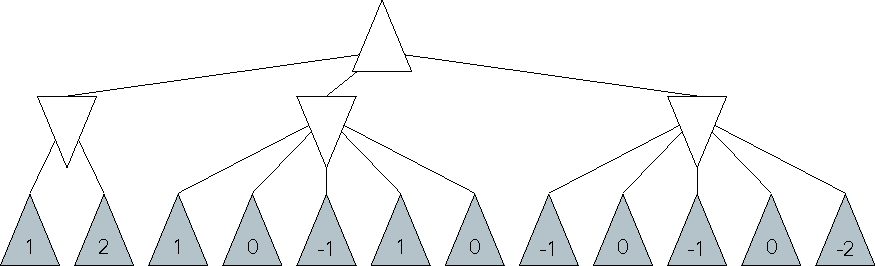
\includegraphics[width=.8\textwidth]{minmax_heuristik.pdf}\\
        & \\
    (b) & 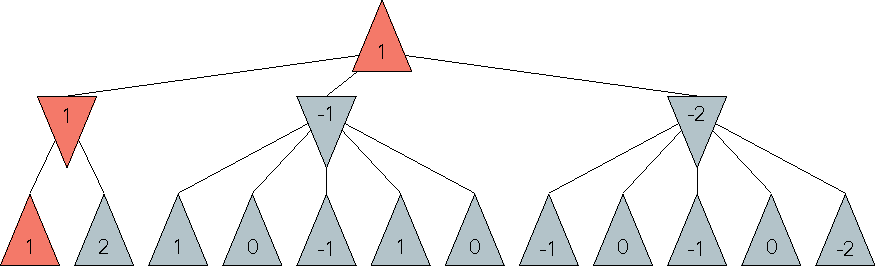
\includegraphics[width=.8\textwidth]{minmax_heuristik_2.pdf}
  \end{tabular}
  \caption{Wenden wir einen Suchbaum der Suchtiefe $t = 2$, ausgehend von der Startkonfiguration des leeren Feldes, aufbauen (vgl. Abb.~\ref{fig:tictactoe}) und dessen Blätter mit der Heuristik $h_1$ bewerten, erhalten wir die geschätzten Werte aus (a), die in (b) im gewohnten Modus zur Wurzel propagiert werden. Der Zug, den \textsc{Max} wählt, ist hervorgehoben.\label{fig:heuristic}}
\end{figure}


\subsection{Alpha-Beta-Pruning}

Um die Komplexität des Minimax-Algorithmus zu verringern, nehmen wir eine weitere Optimierung vor: das \textbf{Alpha-Beta-Pruning}\footnote{erstmals 1956 vorgestellt (\textsc{McCarthy}), auch \q{Alpha-Beta-Kürzung}, \q{$\alpha$-$\beta$-Pruning}, \q{$\alpha$-$\beta$-Cut} oder \q{$\alpha$-$\beta$-Suche}}. Dieses erlaubt es, die Untersuchung von Teilbäumen abzukürzen, ohne dabei aussichtsreiche Züge auszuschließen, indem Knoten nicht weiter expandiert werden (auch, wenn das Expansionskriterium noch erfüllt wäre). 

Dazu führen wir für jeden Knoten $k$ zusätzlich einen \textbf{Alpha-} und \textbf{Beta-Wert} $\alpha_k$ und $\beta_k$ ein. $\alpha_k$ ist dabei die \textit{untere} Schranke des Minimax-Wertes für Max-Knoten und speichert die bisher \textit{größte} Bewertung im Pfad von der Wurzel des aktuellen Suchbaumes zum Knoten $k$. Analog wird in $\beta_k$ die \textit{obere} Schranke für Min-Knoten gespeichert, d.h. die bisher \textit{kleinste} Bewertung im Pfad zu $k$.

Die Alpha- und Beta-Werte werden mit $\alpha = -\infty$, $\beta = +\infty$ initialisiert und nach jeder untersuchten Konfiguration aktualisiert, sodass $\alpha$ an einem Max-Knoten stets maximiert und $\beta$ an einem Min-Knoten stets minimiert wird.

\begin{figure}[!ht]
  \centering
  \begin{tabular}{ll}
    (a) & 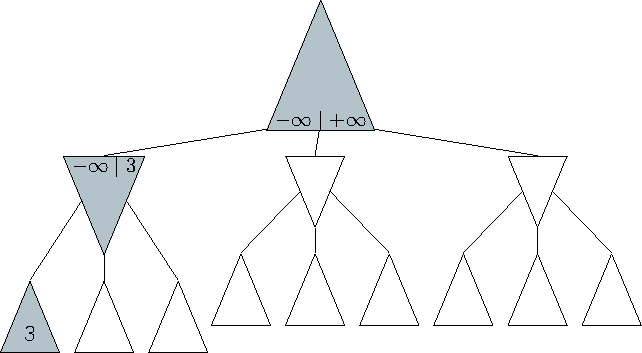
\includegraphics[width=.6\textwidth]{minmax_alphabeta_1.pdf}\\
        & \\
    (b) & 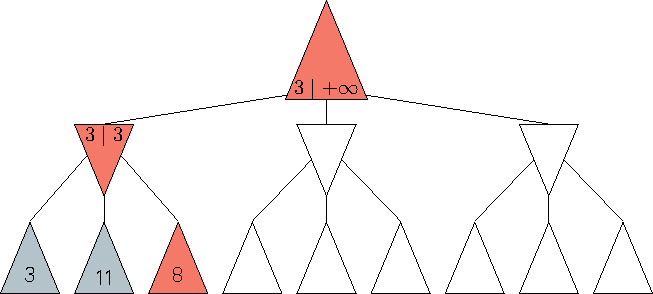
\includegraphics[width=.6\textwidth]{minmax_alphabeta_3.pdf}\\
        & \\
    (c) & 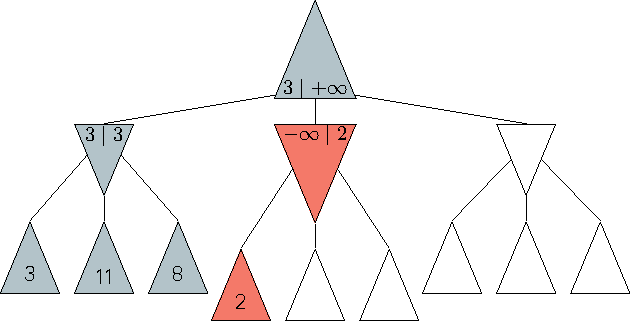
\includegraphics[width=.6\textwidth]{minmax_alphabeta_4.pdf}\\
        & \\
    (d) & 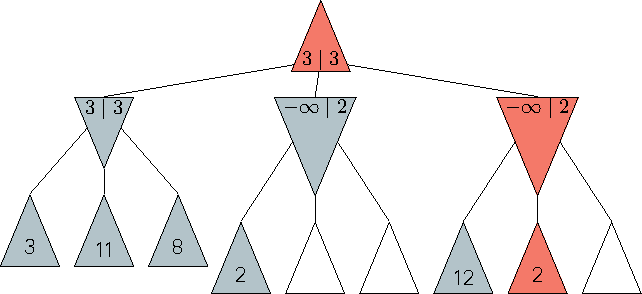
\includegraphics[width=.6\textwidth]{minmax_alphabeta_6.pdf}\\
  \end{tabular}
  \caption{Schrittweiser Ablauf des Alpha-Beta-Prunings; links im Knoten ist der Alpha-, recht der Beta-Wert dargestellt.\label{fig:alphabeta}}
\end{figure}

Wir können nun auf Basis der Alpha- und Beta-Werte \textbf{Kürzungen (Cuts)} vornehmen, d.h. Teilbäume aus dem Suchbaum löschen. Diese können stets durchgeführt werden, sobald sich die beiden Schranken überschneiden. An einem Max-Knoten $u$ -- es wird hier stets der größte Minimax-Wert unter den Kindknoten gesucht --  führen wir den s.g. \textbf{Alpha-Cut} durch, sobald $\exists \beta_v : \beta_v \leq \alpha_u$ ($v \in N(u)$). Analog dazu wird der \textbf{Beta-Cut} an einem Min-Knoten durchgeführt, wenn $\exists \alpha_v : \alpha_v \geq \beta_u$ ($v \in N(u)$).

Dieses formal beschriebene Vorgehen wird durch folgende Überlegung zum Alpha-Cut intuitiver: Da auf einen Max-Knoten stets nur Min-Knoten in der nächsten Ebene des Suchbaumes folgen, müssen diese nicht weiter expandiert werden, wenn bekannt ist, dass ihr Minimax-Wert nie besser werden kann, als der eines bereits untersuchten Min-Knotens (und dessen Teilbaum). Dies ist immer dann der Fall, wenn \e{ein} Minimax-Wert gefunden wird, der den geringsten Wert eines anderen Min-Teilbaumes unterschreitet. Der Beta-Cut, kann analog-umgekehrt genauso verstanden werden.

In Abb.~\ref{fig:alphabeta} kann das Alpha-Beta-Pruning nachvollzogen werden: 

(a) Alpha- und Beta-Werte werden wie beschrieben initialisiert. Der erste Min-Knoten wird expandiert und eine Heuristik angewendet, die den Wert $3$ für den ersten Blattknoten schätzt. Dieser Wert ist damit der Beta-Wert dieses Min-Knotens, da kein kleinerer Wert bisher gefunden wurde. 

(b) Da die Bewertungen beider anderer Blattknoten größer als $3$ ist, ändert sich $\beta$ nicht, und auch $\alpha$ wird auf $3$ gesetzt. Damit erhalten wir im Startknoten $\alpha = 3$, da wir mindestens diesen ersten Kindknoten wählen könnten. Es müssen im Folgenden nur noch Min-Knoten weiter untersucht werden, die einen größeren Wert annehmen können. 

(c) Im zweiten Teilbaum wurde ein Blattknoten mit $2$ bewertet. Das bedeutet, dass der Min-Knoten keinen Wert $> 2$ mehr liefern kann. Dies kann daran abgelesen werden, dass der Beta-Wert dieses Min-Knotens den Alpha-Wert, des darüber liegenden Knotens unterschreitet. Für die verbleibenden beiden Blattknoten (ggf. inklusive ihrer Teilbäume) wird jetzt ein Alpha-Cut durchgeführt und sie müssen nicht untersucht werden. 

(d) Im letzten Teilbaum wiederholt sich dieser Fall, allerdings erst, sobald ein Wert $< \alpha$ geschätzt wird, also beim zweiten Blattknoten. Da nun alle Min-Knoten untersucht wurden, kann auch der Beta-Wert des Wurzelknotens auf $3$ gesetzt werden. Letztendlich wurden in diesem Beispiel drei Kürzungen durchgeführt.

Die Zeitkomplexität sinkt mit dieser Optimierung im besten Fall, d.h. bei optimaler Sortierung der Kindknoten, auf $\mathcal{O}(b^{\frac{m}{2}})$. Dies ist allerdings nur das theoretisches Limit, falls immer sofort gekürzt werden kann. Bei einer zufälligen Sortierung der Knoten erhalten wir eine Zeitkomplexität von $\mathcal{O}(b^{\frac{3}{4}m})$.


\section{Zusammenfassung}

Wir haben den Grundlegenden Minimax-Algorithmus kennengelernt und festgestellt, dass dieser ohne Optimierungen nicht echtzeitfähig ist. Mit dem Alpha-Beta-Pruning wurde eine der wesentlichen Optimierungen vorgestellt.

Es ist nicht auszuschließen, dass in dadurch nicht untersuchten Teilbäumen ein höherer Gewinn für \textsc{Max} zu finden wäre, allerdings hätte auch eine vollständige Suche ohne Kürzungen diesen Zug nie ausgewählt. Grund dafür ist die Eigenschaft des Minimax-Algorithmus', keinerlei Risiko einzugehen. Die mit Alpha-Beta-Kürzung optimierte Variante wird also stets die selben Ergebnisse, wie das bisherige Minimax-Verfahrens liefern. Wir sparen uns lediglich weitere Untersuchungen des Suchbaumes, wenn sich Teilergebnisse ohnehin nicht mehr ändern können.

Natürlich kann man das Verfahren noch weiter verbessern, so ist die Zugreihenfolge für das Alpha-Beta-Pruning entscheidend. Mit bspw. der iterativen Tiefensuche könnte man diese günstig wählen und darüber hinaus auch ggf. begrenzte Zeit best möglich ausnutzen.

Weitere Fragen und Erweiterungen des Szenarios lassen noch Raum zur Vertiefung dieses Themas und müssen hier leider offen bleiben: Was passiert, wenn Zufall im Spiel ist? Wie können wir Spiele mit mehr als zwei Spielern abbilden? Und wie lassen sich Allianzen zwischen mehreren Spielern modellieren?


\begin{thebibliography}{99}
  \bibitem{klueppel:2016} \textsc{Sascha Klüppelholz}
  \newblock \q{Entwurfs- und Analysemethoden für Algorithmen -- Skript zur Vorlesung}, Sommersemester 2016
  \bibitem{russel:2012} \textsc{Russel, Norvig}
  \newblock \q{Künstliche Intelligenz -- Ein moderner Ansatz}, 3., aktualisierte Auflage, 2012
  \bibitem{zermelo:1913} \textsc{Ernst Zermelo}
  \newblock \q{Über eine Anwendung der Mengenlehre auf die Theorie des Schachspiels}, 1913
\end{thebibliography}


\vspace{4\baselineskip}
Diese Ausarbeitung und zugehörige Präsentation sind auch auf github zu finden: \\\url{https://github.com/foobar0112/tic}.

\end{document}